\documentclass[11pt]{article}
\usepackage{fullpage}
\usepackage{amsmath,amsfonts,amsthm,amssymb}
\usepackage{url}
\usepackage{graphicx}
\usepackage{caption} 
\usepackage{algpseudocode}
\usepackage{bbm}
\usepackage{float}
\usepackage{framed}
\usepackage{enumerate}
\usepackage{color}
\usepackage[colorlinks=true, linkcolor=red, urlcolor=blue, citecolor=blue]{hyperref}
\newcommand{\bs}[1]{\mat{#1}}
\newcommand{\bv}[1]{\vec{#1}}

\DeclareMathOperator*{\E}{\mathbb{E}}
\let\Pr\relax
\DeclareMathOperator*{\Pr}{\mathbb{P}}
\DeclareMathOperator*{\R}{\mathbb{E}}
\DeclareMathOperator{\var}{Var}

\topmargin 0pt
\advance \topmargin by -\headheight
\advance \topmargin by -\headsep
\textheight 8.9in
\oddsidemargin 0pt
\evensidemargin \oddsidemargin
\marginparwidth 0.5in
\textwidth 6.5in

\parindent 0in
\parskip 1.5ex

\newcommand{\homework}[2]{
	\noindent
	\begin{center}
		\framebox{
			\vbox{
				\hbox to 6.50in { {\bf NYU CS-GY 9223D: Algorithmic Machine Learning 
						and Data Science} \hfill Fall 2020 }
				\vspace{4mm}
				\hbox to 6.50in { {\Large \hfill Homework #2  \hfill} }
				\vspace{2mm}
				\hbox to 6.50in { {Name: #2 \hfill} }
			}
		}
	\end{center}
	\vspace*{4mm}
}

\begin{document}
	
	\homework{1}{2 Solution key}
	
	\section*{Problem 1}
	\smallskip\noindent 1.\hspace{1em} 
	Once there are $n+1$ servers in this setup, the expected number of items on the $(n+1)^\text{st}$ server is $\frac{m}{n+1}$, by symmetry. All of these items (and only these items) must have been relocated when the $(n+1)^{\text{st}}$ server was added. So the expected number of items that move is $\frac{m}{n+1}$. 
	
	\smallskip\noindent 2. \hspace{1em} For a server $S$ to own more than a $c\log n/n$ fraction of the interval , it would need to be that \emph{no other server} falls within distance $c\log n/n$ to the left of the server. We can choose the random location of server $S$ first. Then the probability of any one server landing within distance $c\log n /n$ from $S$'s left is $c\log n / n$. So the probability \emph{no servers} land that close is:
	\begin{align*}
		(1 - c\log n / n)^{n-1} \leq \frac{1}{10n},
	\end{align*}
	as long as we choose $c$ to be a large enough constant (same analysis as homework 1). By a \emph{union bound}, we thus have that no server owns more than an $O(\log n / n)$ fraction of the interval with probability $\geq 1 - n\frac{1}{10 n} = \frac{9}{10}$ which proves the claim.
	
	\smallskip\noindent 3. \hspace{1em}
	From Part 2, we could have equivalently proven that no server owns more than a $c\log n / n$ fraction of the interval with probability $19/20$ (by choosing $c$ larger). For the rest of the problem, assume that this event happening.
	
	For servers $S_1, \ldots, S_n$ let $Y_i^{(j)}$ be the indicator random variable that item $j$ lands within distance $c\log n / n$ to $S_i$'s left. 
	Let $X_i$ equal $X_i = \sum_{j=1}^m Y_i^{(j)}$.
	Since we assumed that no server owns more than a $c\log n / n$ fraction of the interval, $X_i$ is an \emph{upper bound} on the number of items assigned to server $i$. So it suffices to show that $X_i$ is not too large for all $i$. 
	
	To do so, note that, for a fixed $i$,  $Y_i^{(1)}, Y_i^{(2)}, \ldots, Y_i^{(m)}$ are an independent $\{0,1\}$ random variables, where each is $1$ with probability exactly $c\log n / n$. So they are just biased coin flips!
	
	Let $c > 2$ be a sufficiently large constant. Using the Chernoff bound from class with $\epsilon = c$, we get that:
	\begin{align*}
		\Pr[X_i \geq 2c \cdot \frac{m\log n}{n}] \leq e^{\frac{-c^2m\log n / n}{2+c}} \leq e^{\frac{-c\log n}{2}} \leq \frac{1}{20n}, 
	\end{align*}
	for large enough $c$. The last inequality uses that $m > n$ (as specified in the problem).
	
	We conclude via a union bound that no server is assigned more than $O(m\log n /n)$ items with probability $\frac{19}{20}$. 
	
	There's one last step -- we needed two events to hold for our proof to go through: 1) no server owns more than a $c\log n / n$ fraction of the interval and 2) no server was assigned two many items. Since each holds with probability $19/20$, by another union bound, both hold with probability $9/10$.
	
	\section*{Problem 2 (a)}

1. \textbf{Expectation Calculation.} As in class, we have that $\E[\|\Pi x\|_2^2] =  \E[\langle \pi, x\rangle^2]$, where $\pi$ is a single unscaled row from the matrix $\Pi$. I.e. $\pi$ has length $n$ and contains random $\pm 1$ entries. We have:
\begin{align*}
	\E[\langle \pi, x\rangle^2] = \E\left[\left(\sum_{j=1}^n \pi_j x_j \right)^2\right] &= \E\left[\sum_{j=1}^n \pi_j^2 x_j^2\right] + \E\left[\sum_{i\neq j}^n \pi_i\pi_j x_jx_i \right]\\
	&= \sum_{j=1}^n \E\left[\pi_j^2 \right] x_j^2 +\sum_{i\neq j}^n  \E\left[\pi_i\pi_j\right] x_jx_i .
\end{align*}
The last equality follows from linearity of expectation. Since $\pi_i$ is independent of $\pi_j$, we have that for $j\neq i$, $\E\left[\pi_i\pi_j\right] = \E[\pi_i]\E[\pi_j] = 0$. On the other hand $\pi_j^2 = 1$ deterministically, so we have $\E\left[\pi_j^2 \right]  = 1$. Plugging in above, we find that 
\begin{align*}
	\E[\langle \pi, x\rangle^2] = \sum_{j=1}^n x_j^2 +\sum_{i\neq j}^n  0\cdot x_jx_i  =  \sum_{j=1}^n x_j^2 = \|x\|_2^2,
\end{align*}
as desired.

 \textbf{Variance Calculation.} Since $\|\Pi x\|_2^2 = \frac{1}{k}\sum_{i=1}^k \langle \pi^i, x\rangle^2$, where $\pi^1, \ldots, \pi^k$ are the unscaled rows of $\Pi$, we first observe that $\var[\|\Pi x\|_2^2 ] = \frac{1}{k}\var[\langle \pi, x\rangle^2]$ for a single random $\pm 1$ vector $\pi$. So we just need to bound $\var[\langle \pi_i, x\rangle^2]$. This gets a bit tricky! There are many ways to do it, but I think the easiest way is to take advantage of linearity of variance by writing:
 \begin{align*}
 	\langle \pi, x\rangle^2 = \sum_{j=1}^n \pi_j^2 x_j^2 + 2\sum_{i> j} \pi_i\pi_j x_ix_j. 
 \end{align*}
The terms in the first part of the sum are actually deterministic, since $\pi_j = 1$. The terms in the second part of the sum are random, but they are \emph{pairwise independent} since $\pi_i\pi_j$ is random $\pm 1$ and independent from any $\pi_i\pi_k$, $\pi_k\pi_j$, or $\pi_k\pi_{\ell}$. They are not mutually independent, but we only need pairwise independence to apply linearity of variance. 
Note that to make this claim it's important that I used the form $2\sum_{i> j}$ instead of $\sum_{i\neq j}$. If I did the later, there would be repeated random variables in the sum ($\pi_i\pi_j x_ix_j$  and $\pi_j\pi_i x_jx_i$). Writing the other way removes duplicates.
\begin{align*}
	\var[\langle \pi, x\rangle^2] = \sum_{j=1}^n \var[\pi_j^2 x_j^2] + 4\sum_{i> j} \var[\pi_i\pi_j x_jx_i] = 0 + 4\sum_{i> j} x_j^2x_i^2.
\end{align*}
Then finally we observe that:
\begin{align*}
	\|x\|_2^4 = \|x\|_2^2\cdot \|x\|_2^2 = (x_1^2 + \ldots + x_n^2)\cdot (x_1^2 + \ldots + x_n^2) \geq 2\sum_{i> j} x_j^2x_i^2.
\end{align*} 
Putting this together we have that $\var[\langle \pi, x\rangle^2]  \leq 2 	\|x\|_2^4$ and the result follows since $\var[\|\Pi x\|_2^2 ] = \frac{1}{k}\var[\langle \pi, x\rangle^2]$ as claimed above.

\vspace{.5em}
2. This just follows directly from Chebyshev's.

\vspace{.5em}
3. It's almost the same analysis as in part 1. The first thing to observe is that:
\begin{align*}
	\langle \Pi x, \Pi y\rangle  = \frac{1}{k}\sum_{i=1}^k \langle \pi^i, x\rangle \langle \pi^i, y\rangle. 
\end{align*}
So we have that $\E[\langle \Pi x, \Pi y\rangle] = \E[\langle \pi, x\rangle \langle \pi, y\rangle]$ and $\var[\langle \Pi x, \Pi y\rangle] = \frac{1}{k}\var[\langle \pi, x\rangle \langle \pi, y\rangle]$, where $\pi$ is a single random $\pm 1$ vector. We also have that 
\begin{align*}
	\langle \pi, x\rangle \langle \pi, y\rangle = \left(\sum_{j=1}^n \pi_j x_j \right)\cdot  \left(\sum_{j=1}^n \pi_j y_j \right) = \sum_{i=1}^n\pi_i^2 x_iy_i + \sum_{j\neq i}\pi_i\pi_j x_iy_j.
\end{align*}
From this it's clear that 
\begin{align*}
		\E[\langle \Pi x, \Pi y\rangle]  = \E[\langle \pi, x\rangle \langle \pi, y\rangle] = \sum_{i=1}^n x_iy_i  = \langle x,y\rangle, 
\end{align*}
as desired. 

The variance calculation is also a bit tricky since we need to make sure our sums involve pairwise independent random variables. We have that: 
\begin{align*}
	\langle \pi, x\rangle \langle \pi, y\rangle = \sum_{i=1}^n\pi_i^2 x_iy_i + \sum_{j> i}\pi_i\pi_j (x_iy_j + x_jy_i).
\end{align*}
Applying linearity of variance, we find that 
\begin{align*}
	\var[\langle \pi, x\rangle \langle \pi, y\rangle] = \sum_{j> i} (x_iy_j + x_jy_i)^2 &= \sum_{j> i} x_i^2y_j^2 + x_j^2y_i^2  + 2 x_ix_jy_iy_j \\
	&\leq 2 \sum_{j> i} x_i^2y_j^2 + x_j^2y_i^2 \\
	& \leq 2(x_1^2 + \ldots + x_n^2)(y_1^2 + \ldots + y_n^2) \\
	&= 2 \|x\|_2^2 \|y\|_2^2.
\end{align*}
In second to last inequality we have used that for any $a,b$, $2ab \leq a^2 + b^2$, which follows from the fact that $(a-b)^2 \geq 0$ for all $a,b$ (this is technically called the AM-GM inequality).

Overall, we get a variance bound of:
\begin{align*}
	\var[\langle \Pi x, \Pi y\rangle] \leq \frac{2}{k}\|x\|_2^2 \|y\|_2^2.
\end{align*}

Once they get the mean and variance, the bound just follows from applying Chebyshev inequality again.
	.
	\section*{Problem 2 (b)}
	1. Construct 2 length $U$ binary vectors $x$ and $y$ where $x_i = 1$ if $i \in X$ and $0$ otherwise, and $y_i = 1$ if $i \in Y$ and $0$ otherwise. Note that $|X\cap Y|$ is exactly equal to $\langle x, y\rangle$, so we can estimate the quantity using sketches $\Pi x$ and $\Pi y$. If we set $k = O(1/\epsilon^2)$, then with $9/10$ probability we will have:
	\begin{align*}
		\left|\langle  x, y \rangle  - \langle \Pi x, \Pi y \rangle \right| \leq \epsilon \|x\|_2 \|y\|_2
	\end{align*}
Note that $\|x\|_2^2 = |X|$ and $\|y\|_2^2 = |Y|$, which yields the bound. 

\vspace{.5em}

	
	\section*{Problem 3}
	\smallskip\noindent 1.\hspace{1em}
	For any vector $x$, let $z$ be the point on the hyperplane closest to $x$. Now: 
	\begin{align*}
	\langle x, a \rangle = \langle x - z, a \rangle  + \langle z, a \rangle  = \langle x - z, a \rangle +c = \|x - z\|_2 + c \geq c + \epsilon.
	\end{align*}
In the second step we used that  $\langle z, a \rangle =c$ since $z$ is on the hyperplane. And in the next step we use that $x - z$ must be perpendicular to the hyperplane (for $z$ to be the closest point). And thus $x - z$ is \emph{parallel} to $a$. Since $a$ is a unit vector, $\langle x - z, a \rangle= \|x-z\|_2$. The proof for any $y$ on the other size of the hyperplane is the same, but in that case, $y-z$ points directly opposite of $a$
	
	\smallskip\noindent 2.\hspace{1em}	
	To show that there exists a good separating hyperplane for the dimension reduced data, we  exhibit one: consider the hyperplane given by parameters $\Pi a/\|\Pi a\|_2 , c/\|\Pi a\|_2$. 
	
	We can apply Problem 2 to claim that, if $\Pi$ reduces to $O(\log(1/\delta)/\epsilon^2)$ dimensions, then with probability $(1-\delta)$ for \emph{any} $x \in X$ or $\forall y \in Y$,
	\begin{align*}
	\langle \Pi a, \Pi x \rangle &\geq \langle a, x \rangle - \epsilon/2 \geq c + \epsilon/2 & &\text{and} & \langle \Pi a, \Pi y \rangle &\leq \langle a, y \rangle + \epsilon/2 \leq c - \epsilon/2.
	\end{align*}
	Above we use the fact that $\|x\|_2\|\bv{a}\|_2 = 1$ and $\|y\|_2\|\bv{a}\|_2 = 1$ since all $x$ and $y$ are specified to be unit vectors. Equivalently, we have:
	\begin{align}
	\label{eq:4}
	\langle \Pi a/\|\Pi a\|_2, \Pi x \rangle &\geq c/\|\Pi a\|_2 + \epsilon/2\|\Pi a\|_2 & &\text{and} & \langle \Pi a/\|\Pi a\|_2, \Pi y \rangle &\geq c/\|\Pi a\|_2 + \epsilon/2\|\Pi a\|_2.
	\end{align}
	
	
	We also have from the distributional JL lemma that, with probability $1 - \delta$, $\|\Pi a\|_2 \leq 2$. And if we set $\delta = 1/99(n+1)$, by a union bound we have that \eqref{eq:4} holds for all $n$ points in our data set and $\|\Pi a\|_2 \leq 2$ simultaneously with probability $99/100$. This proves the claim with margin $\epsilon/4$. 
	
	\section*{Problem 4}
	This problem can be solved in a similar way to the Shazam example from the Lecture 4 notes. You need to optimize over values of $s$ and $t$, where $s$ is the number of independent locality-sensitive hash functions used in your scheme and $t$ is the number of tables used. 
	
	
	Following the analysis in Lecture 5, given a query vector $\bv{y}$ and some database vector $\bv{x}$, the probability of $\bv{x}$ showing up as a candidate near-duplicate (which will need to be scanned when $\bv{y}$ is issued as a query) is equal to:
	\begin{align}
		(1 - (1 - \theta(\bv{x},\bv{y})/\pi)^s)^t
	\end{align}
	where $\theta$ is the angle between vectors $\bv{x}$ and $\bv{y}$. 
	
	Our goal is to find the $s,t$ pair with the smallest value of $t$ which satisfies:
	\begin{enumerate}
		\item If $\cos(\theta(\bv{x},\bv{y})) \geq .98$, $(1 - (1 - \theta(\bv{x},\bv{y})/\pi)^s)^t \geq .99$
		\item Based on the histogram data provided, the expected number of candidate near-duplicates in less than $1$ million, or $200$k, for parts (1) and (2).
	\end{enumerate}
	
	Observe that $(1 - (1 - \theta(\bv{x},\bv{y})/\pi)^s)^t$ is monotonically decreasing with $s$ and the expected number of duplicates monotonically decreases with $s$. So, for a given value of $t$, it suffices to find the largest possible $s$ such that  $(1 - (1 - \cos^{-1}(.98)/\pi)^s)^t \geq .99$. I did this by solving for:
	\begin{align*}
		s = \frac{\log(1 - (1-.99)^{1/t})}{\log(1-\cos^{-1}(.98)/\pi)}
	\end{align*}
	and taking the floor. 
	
	Then an upper bound on the number of expected candidates can be computed for this $s$. This will be the smallest possible number of expected candidates for the given $t$. 
	
	My code is included below. I obtained solutions of:
	\begin{itemize}
		\item $\mathbf{20}$ \textbf{tables} for $\leq 1$ million candidates
		\item  $\mathbf{44}$ \textbf{tables} for $\leq 200$k candidates
	\end{itemize}
	
	\begin{figure}
	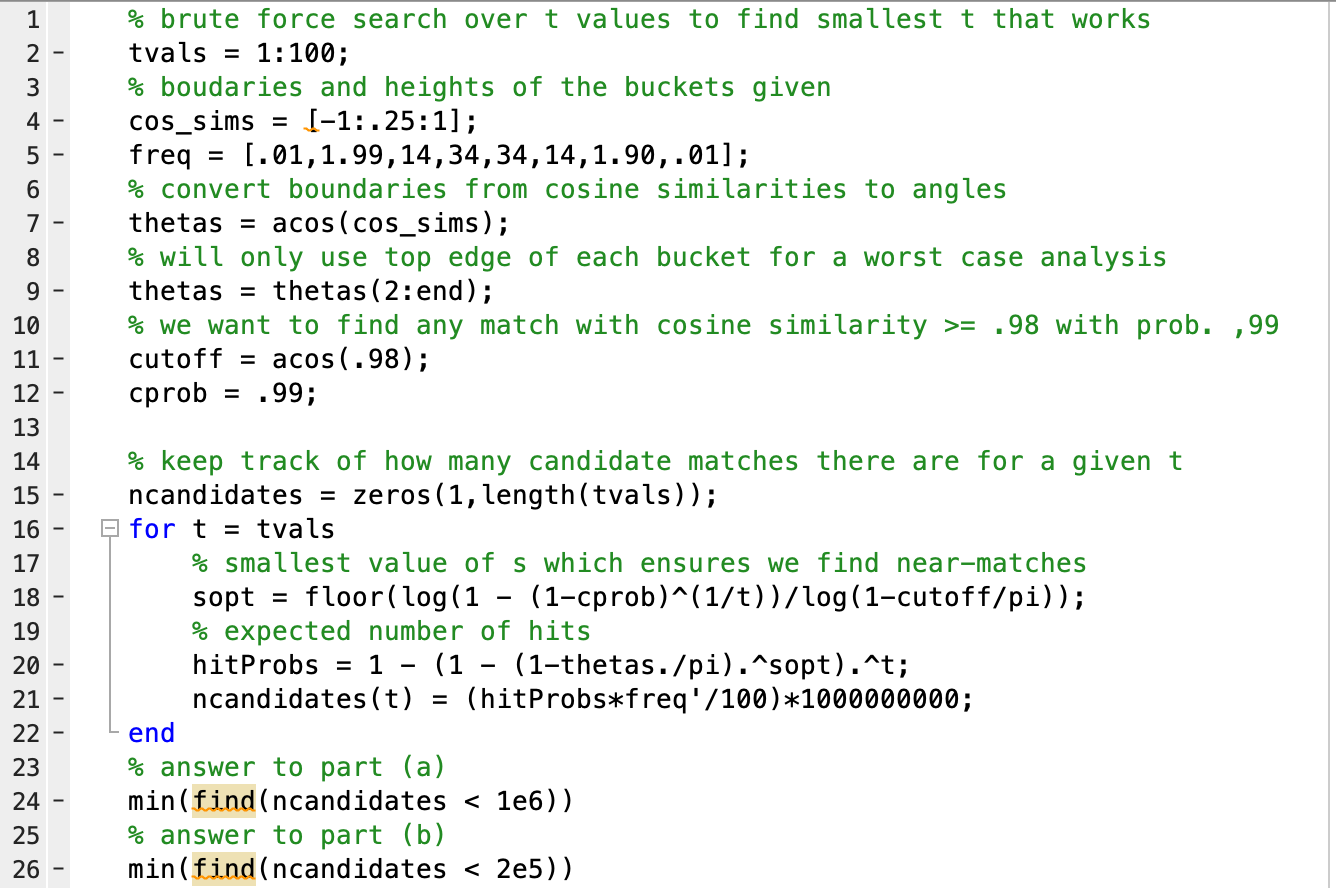
\includegraphics[width=\textwidth]{matlabCode.png}
	\end{figure}
	
\end{document}